
\section{L2 Cache Size Sensitivity}
\label{sec:results:l2size_sensitivity}

\todo{First figure shows how an increasing size of l2 cache causes fewer accesses to l3, and hence all algorithms have fewer request to base their choices on}
\todo{All other figures in general show that when size of private cache incrases, the gains of running a custom algorithm over running lru lessens. By this observation it seems that if the choice is either increasing chache space, or utilizing a more advanced algorithm, then the choice may not be obvious.}

\begin{figure}[H]
    \centering
    \begin{subfigure}[b]{0.5\textwidth}
	    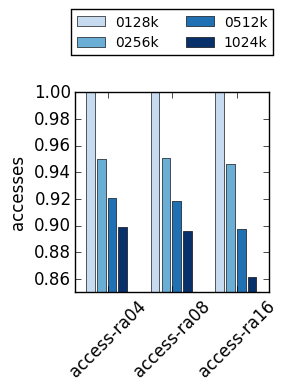
\includegraphics[width=\textwidth]{figures/results/speedup/accesses-accesses-0128k-0100-access}
	    \caption{Relative number of accesses to L3 cache with varying L2 size}
	    \label{fig:results:l2:access}
    \end{subfigure}
    \begin{subfigure}[b]{0.5\textwidth}
        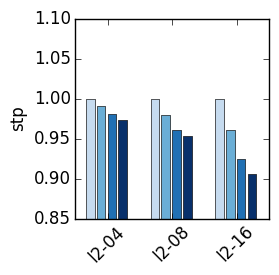
\includegraphics[width=\textwidth]{figures/results/speedup/l2-stp-0128k-tadip-l2}
        \caption{Speedup of TADIP relative to LRU}
        \label{fig:results:l2:tadip}
    \end{subfigure}%
    \begin{subfigure}[b]{0.5\textwidth}
        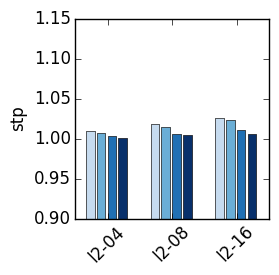
\includegraphics[width=\textwidth]{figures/results/speedup/l2-stp-0128k-drrip-3-l2}
        \caption{Speedup of DRRIP relative to LRU}
        \label{fig:results:l2:drrip}
    \end{subfigure}
\end{figure}
\clearpage
\begin{figure}[H]
	\ContinuedFloat
    \begin{subfigure}[b]{0.5\textwidth}
        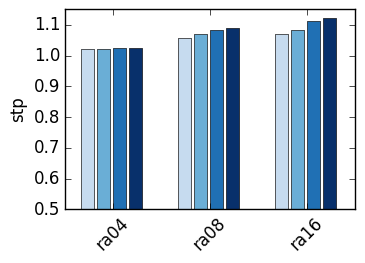
\includegraphics[width=\textwidth]{figures/results/speedup/l2-stp-0128k-ucp-l2}
        \caption{Speedup of UCP relative to LRU}
        \label{fig:results:l2:ucp}
    \end{subfigure}%
    \begin{subfigure}[b]{0.5\textwidth}
        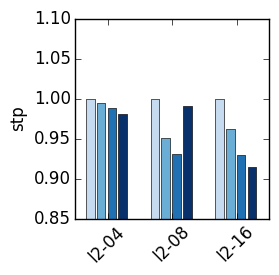
\includegraphics[width=\textwidth]{figures/results/speedup/l2-stp-0128k-prism-l2}
        \caption{Speedup of PriSM relative to LRU}
        \label{fig:results:l2:prism}
    \end{subfigure}
    \begin{subfigure}[b]{0.5\textwidth}
        \includegraphics[width=\textwidth]{figures/results/speedup/l2-stp-0128k-pipp-l2}
        \caption{Speedup of PIPP relative to LRU}
        \label{fig:results:l2:pipp}
    \end{subfigure}%
    \begin{subfigure}[b]{0.5\textwidth}
        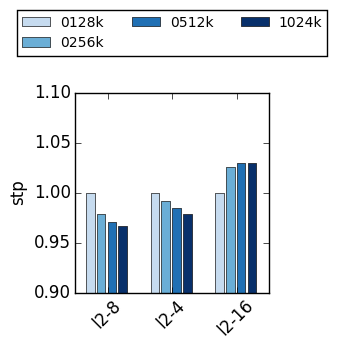
\includegraphics[width=\textwidth]{figures/results/speedup/l2-stp-0128k-pipp-min8-l2}
        \caption{Speedup of PIPP-min8 relative to LRU}
        \label{fig:results:l2:pipp-min8}
    \end{subfigure}
    \caption{Speedup of cache paritition algorithms relative to LRU with increasing private L2 size}
    \label{fig:results:l2}
\end{figure}